\chapter[Planificación y costes]{
  \label{chp:planificacion}
  PLANIFICACIÓN Y COSTES
}
\thispagestyle{numberingStyle}
\pagestyle{numberingStyle}



\section{Planificación}

\subsection{Planificación de las tareas}
Para las iteraciones definidas anteriormente se establecerá una división en tareas, sobre las que se realizará la planificación necesaria para obtener la estimación del esfuerzo requerido en cada iteración.

A continuación, se mostrará las diferentes tareas que componen cada una de las iteraciones junto con los valores del tiempo necesario para su realización (en horas).

\subsubsection*{Iteración 1: Análisis de requisitos y diseño}

\begin{figure}[H]
\vspace{-0.5cm}
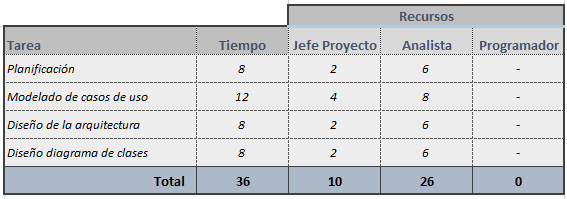
\includegraphics[
   keepaspectratio=true
]{./03_Met_Plan/02_Planificacion/img/PlanIter1.png}
\caption{Diagrama tareas iteración 1}
\end{figure}


\subsubsection*{Iteración 2: Base inicial proyecto}

\begin{figure}[H]
\vspace{-1cm}
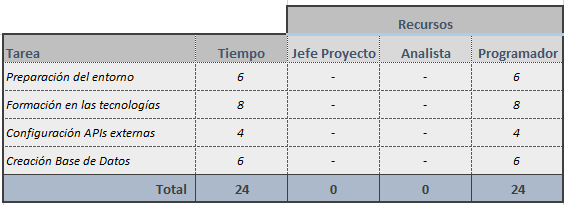
\includegraphics[
   keepaspectratio=true
]{./03_Met_Plan/02_Planificacion/img/PlanIter2.png}
\caption{Diagrama tareas iteración 2}
\end{figure}


\subsubsection*{Iteración 3: Usuarios}

\begin{figure}[H]
\vspace{-1cm}
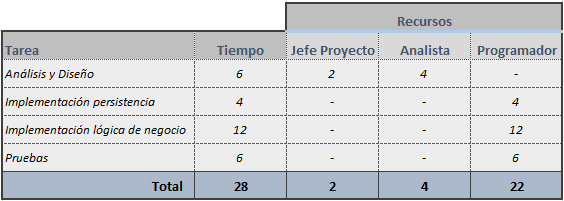
\includegraphics[
   keepaspectratio=true
]{./03_Met_Plan/02_Planificacion/img/PlanIter3.png}
\caption{Diagrama tareas iteración 3}
\end{figure}


\subsubsection*{Iteración 4: Rutas}

\begin{figure}[H]
\vspace{-1cm}
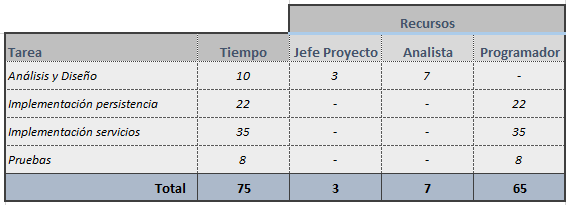
\includegraphics[
   keepaspectratio=true
]{./03_Met_Plan/02_Planificacion/img/PlanIter4.png}
\caption{Diagrama tareas iteración 4}
\end{figure}



\subsubsection*{Iteración 5: Eventos}

\begin{figure}[H]
\vspace{-1cm}
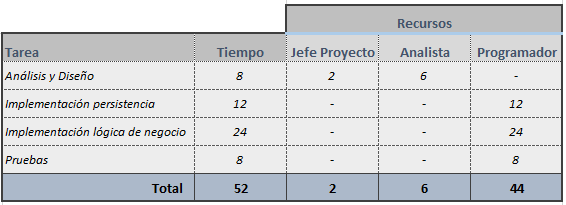
\includegraphics[
   keepaspectratio=true
]{./03_Met_Plan/02_Planificacion/img/PlanIter5.png}
\caption{Diagrama tareas iteración 5}
\end{figure}


\subsubsection*{Iteración 6: Servicios externos}

\begin{figure}[H]
\vspace{-1cm}
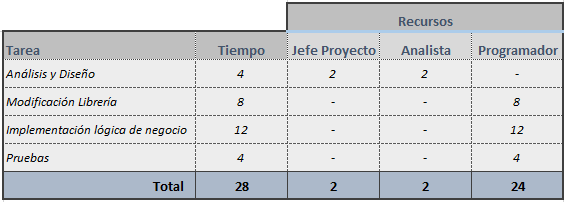
\includegraphics[
   keepaspectratio=true
]{./03_Met_Plan/02_Planificacion/img/PlanIter6.png}
\caption{Diagrama tareas iteración 6}
\end{figure}


\subsubsection*{Iteración 7: Lugares y categorías}

\begin{figure}[H]
\vspace{-1cm}
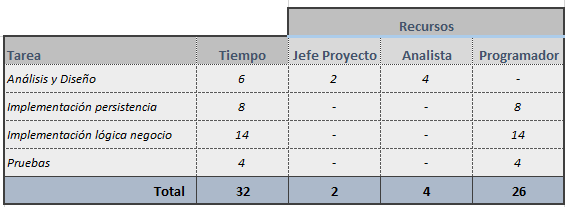
\includegraphics[
   keepaspectratio=true
]{./03_Met_Plan/02_Planificacion/img/PlanIter7.png}
\caption{Diagrama tareas iteración 7}
\end{figure}


\subsubsection*{Iteración 8: Capa servicios}

\begin{figure}[H]
\vspace{-1cm}
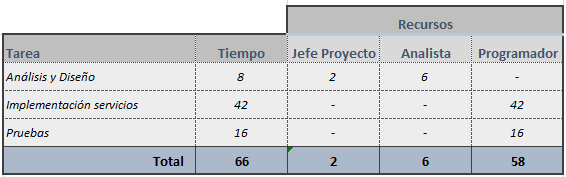
\includegraphics[
   keepaspectratio=true
]{./03_Met_Plan/02_Planificacion/img/PlanIter8.png}
\caption{Diagrama tareas iteración 8}
\end{figure}


\subsubsection*{Iteración 9: Autenticación y autorización}

\begin{figure}[H]
\vspace{-1cm}
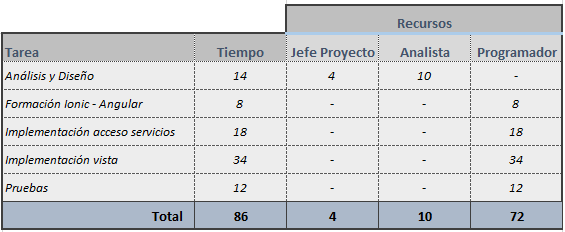
\includegraphics[
   keepaspectratio=true
]{./03_Met_Plan/02_Planificacion/img/PlanIter9.png}
\caption{Diagrama tareas iteración 9}
\end{figure}


\subsubsection*{Iteración 10: Cliente móvil}

\begin{figure}[H]
\vspace{-1cm}
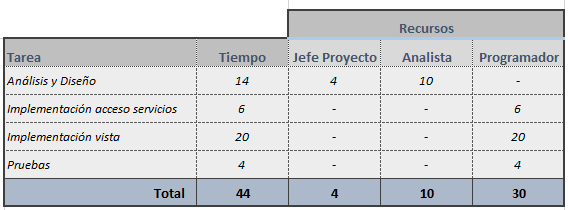
\includegraphics[
   keepaspectratio=true
]{./03_Met_Plan/02_Planificacion/img/PlanIter10.png}
\caption{Diagrama tareas iteración 10}
\end{figure}


\subsubsection*{Iteración 11: Cliente web}

\begin{figure}[H]
\vspace{-1cm}
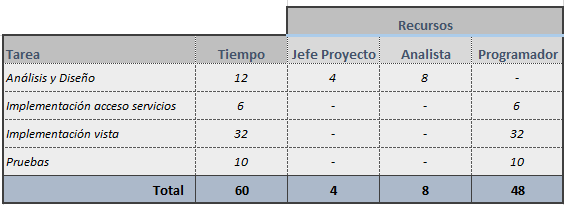
\includegraphics[
   keepaspectratio=true
]{./03_Met_Plan/02_Planificacion/img/PlanIter11.png}
\caption{Diagrama tareas iteración 11}
\end{figure}


\subsubsection*{Iteración 12: Panel de administración}

\begin{figure}[H]
\vspace{-1cm}
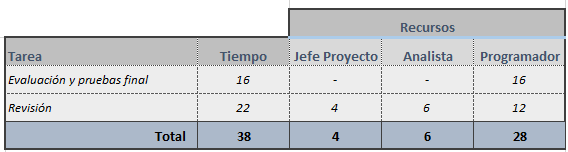
\includegraphics[
   keepaspectratio=true
]{./03_Met_Plan/02_Planificacion/img/PlanIter12.png}
\caption{Diagrama tareas iteración 12}
\end{figure}


\subsubsection*{Iteración 13: Cierre}

\begin{figure}[H]
\vspace{-1cm}
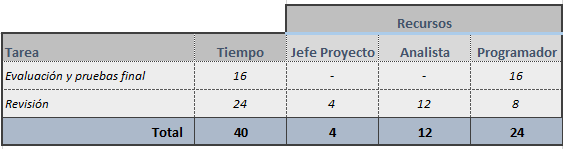
\includegraphics[
   keepaspectratio=true
]{./03_Met_Plan/02_Planificacion/img/PlanIter13.png}
\caption{Diagrama tareas iteración 13}
\end{figure}


\subsubsection*{Planificación global}

\begin{figure}[H]
\vspace{-0.5cm}
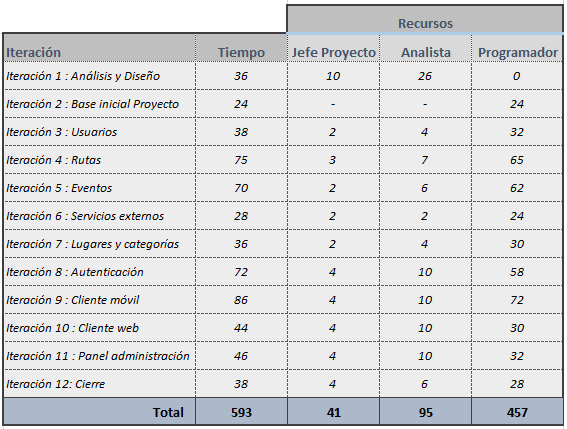
\includegraphics[
   keepaspectratio=true
]{./03_Met_Plan/02_Planificacion/img/PlanIterGlobal.png}
\caption{Diagrama tareas global}
\end{figure}



\subsubsection*{Diagrama de Gantt}
En el siguiente diagrama se podrá observar la planificación establecida en cada iteración, así como, la planificación total del proyecto.

\begin{figure}[H]
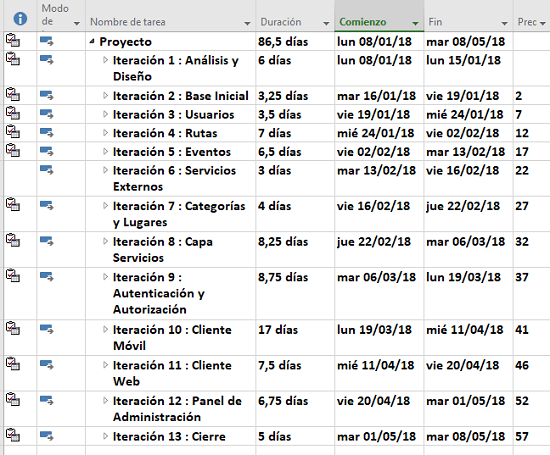
\includegraphics[
   keepaspectratio=true
]{./03_Met_Plan/02_Planificacion/img/gantt1.png}
\caption{Diagrama Gantt - global}
\end{figure}

Observando el diagrama se puede observar la duración, la fecha de comienzo y de fin para cada iteración. En los siguientes diagramas se mostrará la planificación por tareas para cada una de las iteraciones.


\begin{figure}[H]
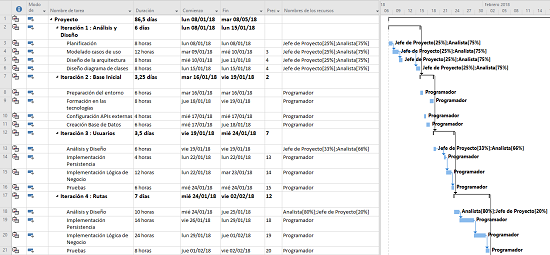
\includegraphics[
   keepaspectratio=true
]{./03_Met_Plan/02_Planificacion/img/gantt2.png}
\caption{Diagrama Gantt - iteraciones 1-4}
\end{figure}

\begin{figure}[H]
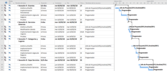
\includegraphics[
   keepaspectratio=true
]{./03_Met_Plan/02_Planificacion/img/gantt3.png}
\caption{Diagrama Gantt - iteraciones 5-8}
\end{figure}

\begin{figure}[H]
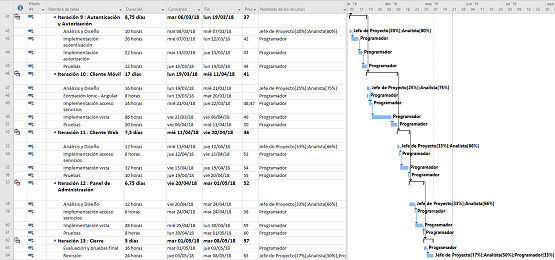
\includegraphics[
   keepaspectratio=true
]{./03_Met_Plan/02_Planificacion/img/gantt4.png}
\caption{Diagrama Gantt - iteraciones 9-13}
\end{figure}

En los diagramas mostrados se puede ver la planificación de las tareas para cada una de las iteraciones, indicando para cada una de ellas, el nombre, la fecha de inicio y fin, la duración, las tareas predecesoras y los recursos asignados encargados de realizar dicha tarea.


\section{Evaluación de costes}
\subsection{Recursos Humanos}
\subsection{Costes Hardware}
\subsection{Costes Software}
\subsection{Costes totales}

